\begin{figure}[htbp]
    \begin{subfigure}{.5\textwidth}
    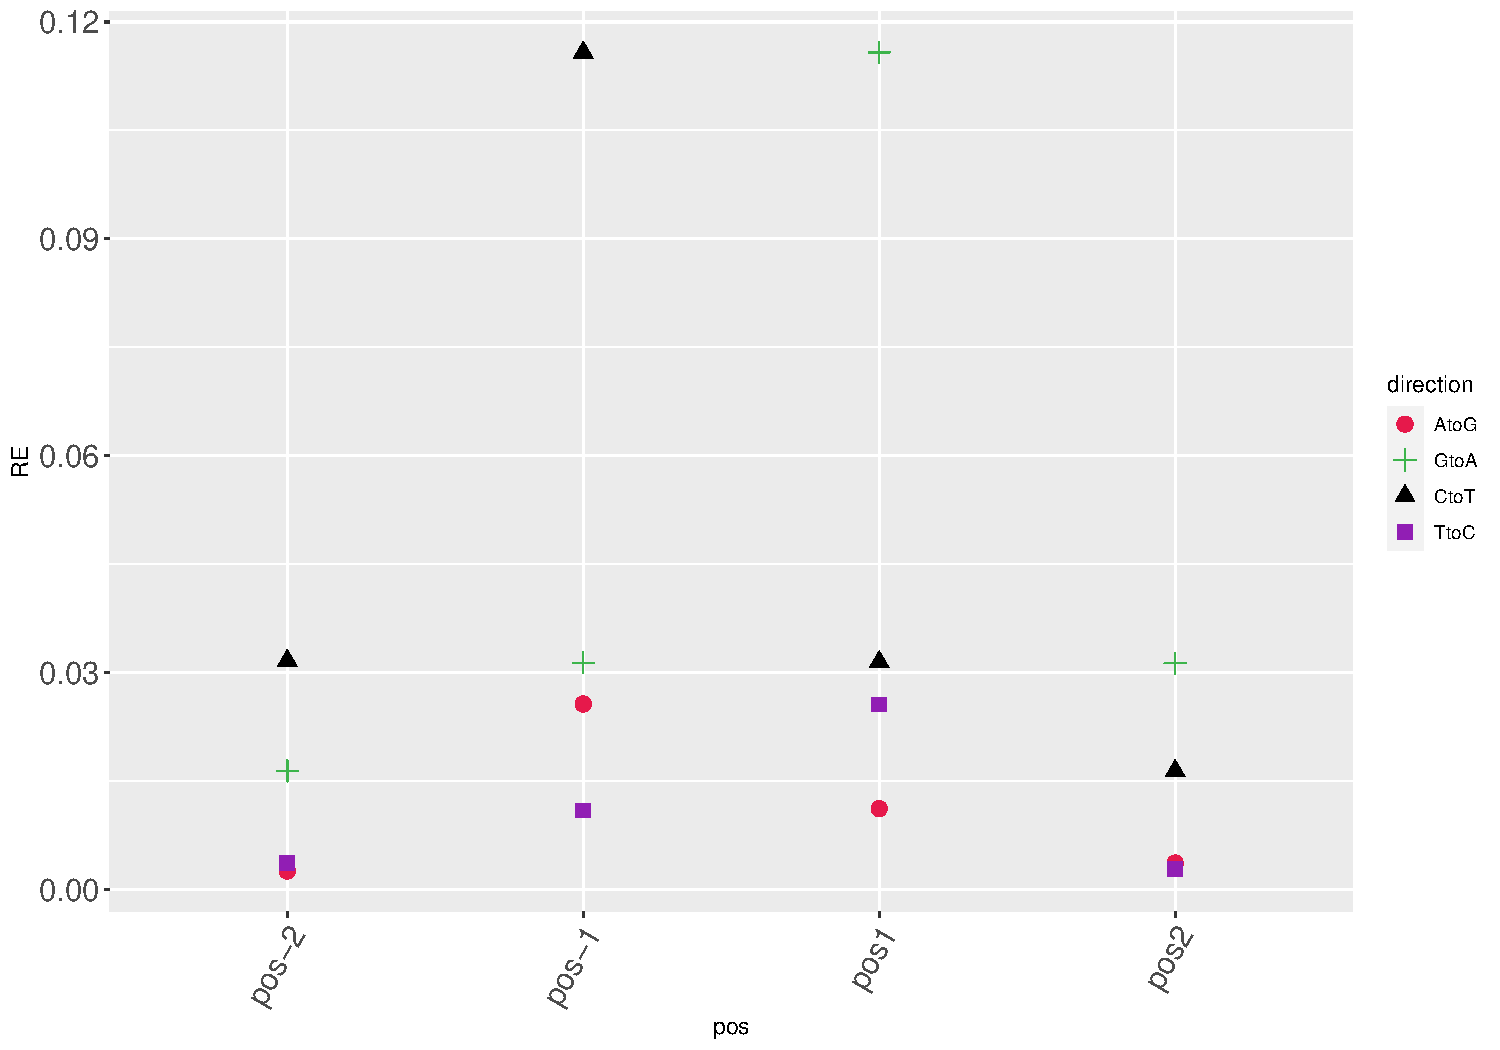
\includegraphics[scale=0.32]{graphics/nbr_transitions_Skin-Melanoma.pdf}
    \caption{transitions/Skin-Melanoma}
    \label{fig:transitions_skin}
    \end{subfigure}
    ~
    \begin{subfigure}{.5\textwidth}
    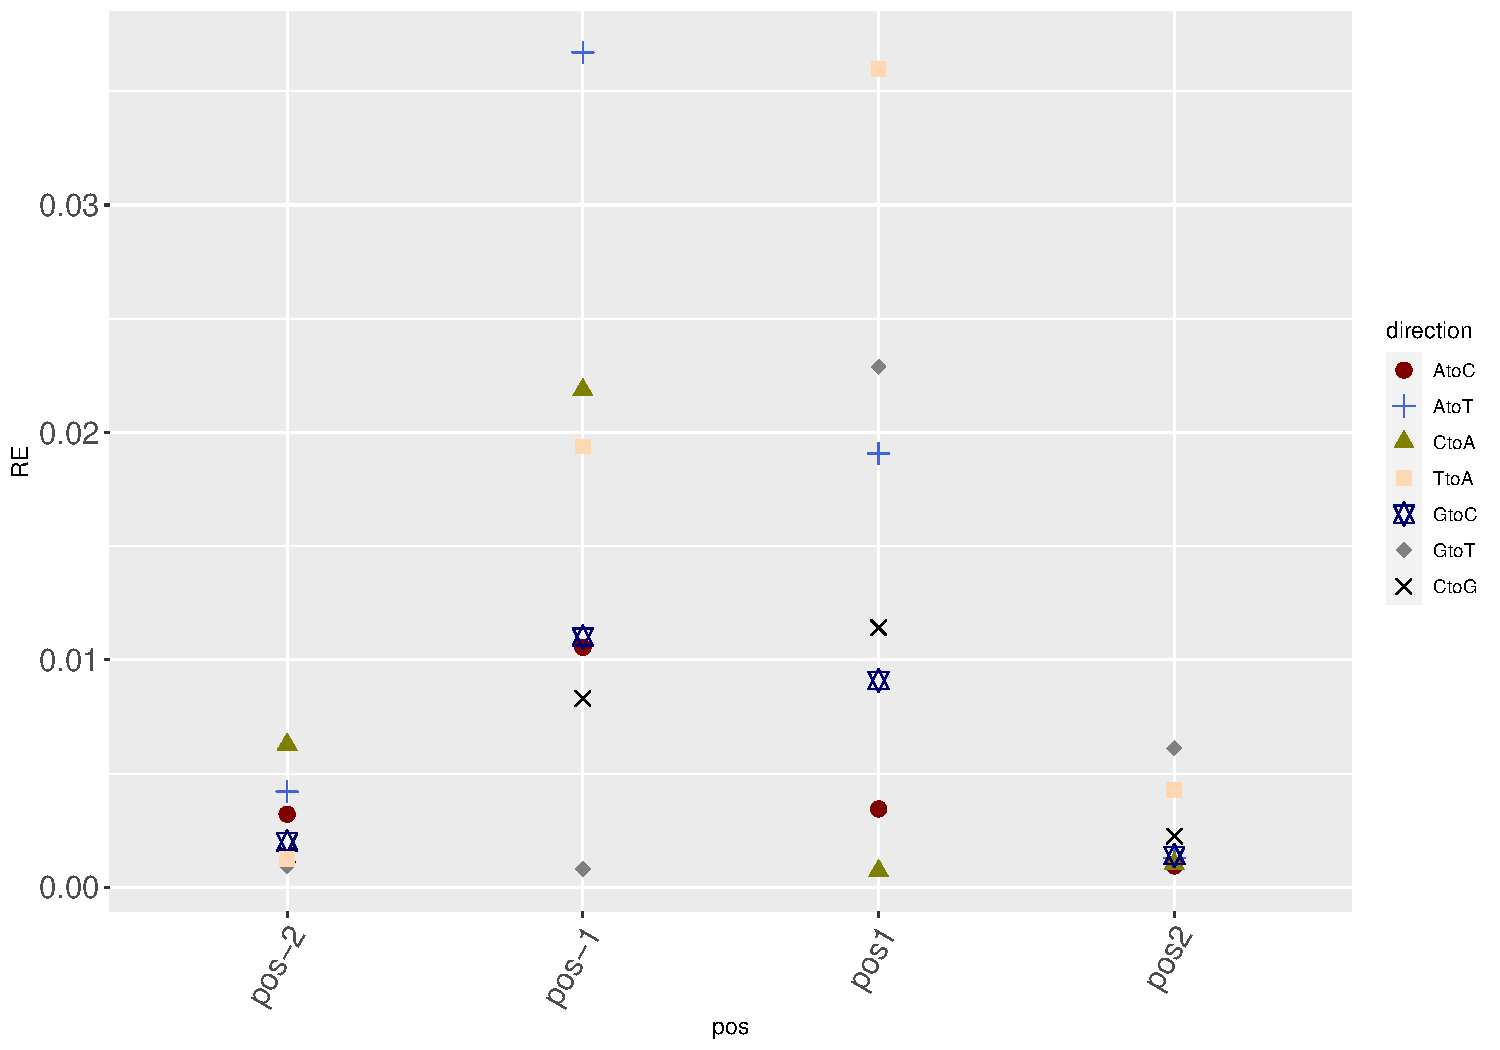
\includegraphics[scale=0.32]{graphics/nbr_transversion_Skin-Melanoma.pdf}
    \caption{transversions/Skin-Melanoma}
    \label{fig:transversions_skin}
    \end{subfigure} \\
    \vspace{0.5cm}
    
    \begin{subfigure}{.5\textwidth}
    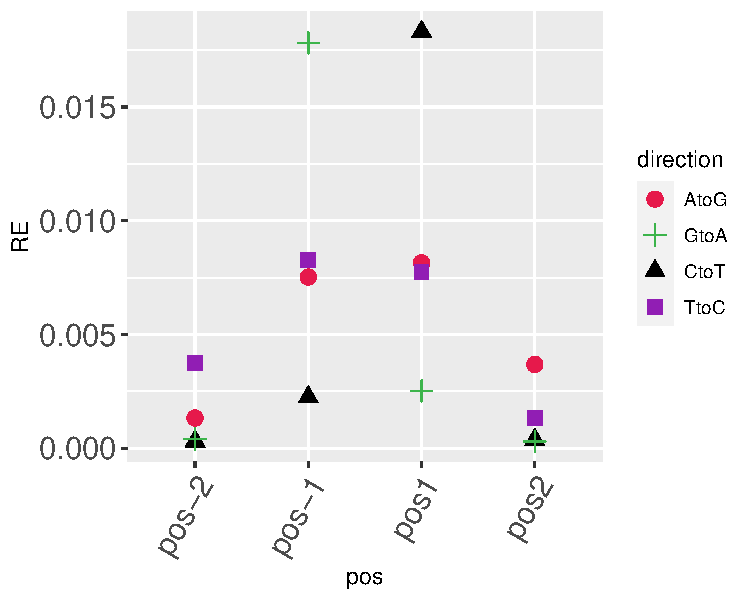
\includegraphics[scale=0.32]{graphics/nbr_transitions_Liver-HCC.pdf}
    \caption{transitions/Liver-HCC}
    \label{fig:transitions_liver}
    \end{subfigure}
    ~
    \begin{subfigure}{.5\textwidth}
    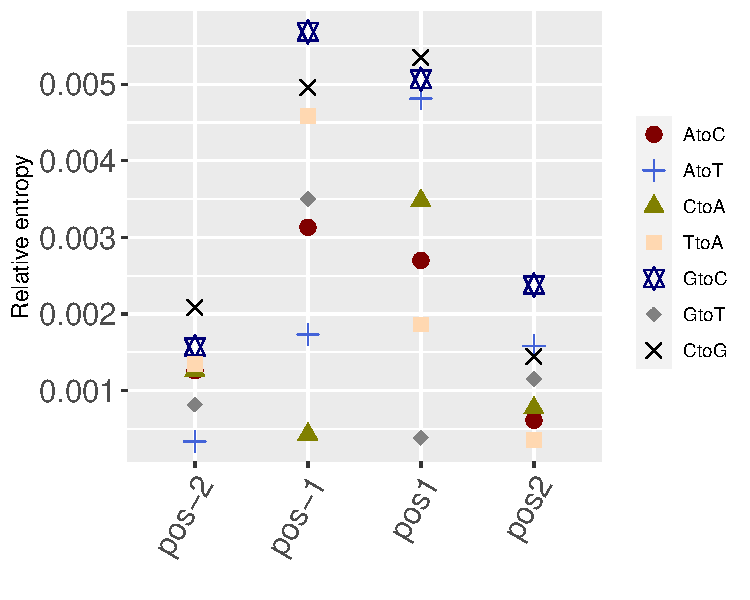
\includegraphics[scale=0.32]{graphics/nbr_transversion_Liver-HCC.pdf}
    \caption{transversion/Liver-HCC}
    \label{fig:transversion_liver}
    \end{subfigure} \\
    
    \caption{\textbf{Flanking bases are a good source of information, according to $RE$}. Here, $RE$'s are shown for (a) transitions in Skin-Melanoma (b) transversions in Skin-Melanoma (c) transitions in Liver-HCC (d) transitions in Liver-HCC. For each panel, each dot was derived from a GLM. The x-axis is the flanking positions with respect to the substitution (substitution at 0); the y-axis is the $RE$ values.}
    \label{fig:nbr}
\end{figure}